\documentclass[handout]{beamer}

\usetheme[progressbar=frametitle]{metropolis}
\metroset{block=fill}

\subtitle{NTIN071 Automata and Grammars}
\author{Jakub Bulín (KTIML MFF UK)}

\date{Spring 2025\\ 
    \vspace{1in} 
    \begin{flushleft}
        \it \footnotesize * Adapted from the Czech-lecture slides by Marta Vomlelová with gratitude. The translation, some modifications, and all errors are mine.
    \end{flushleft}
}

%% packages

\usepackage{amsmath}
\usepackage{amssymb}
\usepackage{amsthm}
\usepackage{cancel}
\usepackage{color}
\usepackage{colortbl}
\usepackage{forest}
\usepackage[utf8x]{inputenc}
\usepackage{multicol}
\usepackage{multirow}

%% colors
\definecolor{Gray}{gray}{0.9}

%% TikZ
\usepackage{tikz}
    \usetikzlibrary{
        automata,
        arrows,
        backgrounds,
        decorations.pathmorphing,
        fit,
        positioning,
        shapes,
        shapes.geometric,
        tikzmark
    } 
    \tikzset{>=stealth',shorten >=1pt,auto,node distance=2cm}
    \tikzset{initial text={}}
    \tikzset{elliptic state/.style={draw,ellipse}}

%% amsthm
\theoremstyle{plain}
    \newtheorem*{algorithm}{Algorithm}    
    \newtheorem*{observation}{Observation}
    \newtheorem*{proposition}{Proposition}

\theoremstyle{remark}
    \newtheorem*{exercise}{Exercise}
    \newtheorem*{remark}{Remark}

%% macros
\DeclareMathOperator{\RegE}{RegE}
\DeclareMathOperator{\RL}{RL}

% Just for Lecture 2
\newcommand{\x}{$\times$}
\newcommand{\nx}{\ }



\title{Lecture 1 -- Deterministic Finite Automaton, Regular Languages, Pumping Lemma}


\begin{document}


\frame{\titlepage}


\section{About the course}


\begin{frame}{The path to success}

    \begin{itemize}    
        \item \alert{Study and self-test regularly (ideally each week).} Can you write down the definition/theorem/proof, fully and correctly?
        \item \alert{Make your own notes.} The slides are not fully self-contained.
        \item \alert{Review after each lecture.} Complete your understanding.
        \item \alert{Try to attend all lectures.} If you miss one, catch up before the next. Use office hours and the textbooks as needed.
        \item \alert{Learn to work with the formalism,} comfortably and precisely.
        \item \alert{Pay attention to the tutorial} in a similar way.

    \end{itemize}

\end{frame}


\begin{frame}{Aims of the course}

    \begin{itemize}
        \item get familiar with abstract models of computation
        \item be able to \alert{formally} describe such models
        \item understand how minor changes can lead to huge difference in expressive power
        \item experience the unavoidability of undecidable problems
        \item prepare for NTIN090 Intro to Complexity and Computability
        \item also used in NSWI098 Compiler Principles, and in linguistics
    \end{itemize}
    
    Two levels of understanding: the \alert{idea} behind a concept and the ability to \alert{formalize} said concept

\end{frame}


\begin{frame}{Resources}

    The course is mostly based on the following two textbooks:

    \begin{itemize}
        \item \alert{Hopcroft} et al: ``Introduction to Automata Theory, Languages, and Computation'' (3rd edition) -- an online copy and several physical copies are available in the library
        \item \alert{Sipser}: ``Introduction to the theory of computation'' (3rd edition) -- a physical copy is in the library
    \end{itemize}    

\end{frame}


\section{\sc Introduction}


\begin{frame}{Formal languages}

    A \alert{language} $L$ over an \alert{alphabet} $\Sigma$ is a set of \alert{words} (finite strings) consisting of symbols (letters) from the alphabet. 

    Languages can represent:
    \begin{itemize}
        \item natural languages (words, well-formed sentences), 
        \item programming languages (expressions, statements), document formats (XML,\dots)
        \item formal proofs
        \item possible strings of input or sensor readings of a machine, or 
        \item \alert{decision problems}, for example, $\Sigma = \{0, 1\}$ and 
        $$L = \{w \in \Sigma^\star\mid w\text{ encodes a CNF formula which is satisfiable}\}$$
    \end{itemize}

\end{frame}


\begin{frame}{Classifying languages}

    \begin{itemize}
        \item Testing (membership of) words: how complex is the computing device needed? (\alert{automata})
        \item Generating words: how complex rules? (\alert{grammars})
    \end{itemize}

    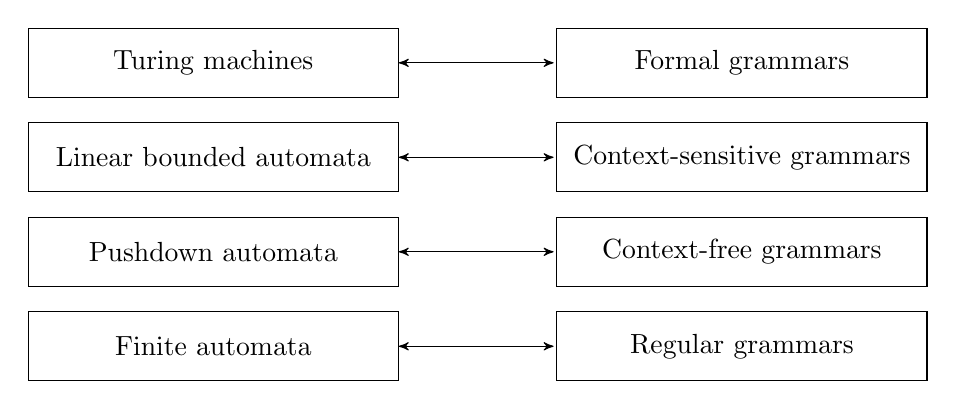
\begin{tikzpicture}[node distance=1.2cm]
        \node[state,rectangle, minimum width =4.7cm][align=center] (fa)      {\alert{Finite automata}};
        \node[state,rectangle, minimum width =4.7cm] (pda) [above of=fa]  {Pushdown automata};
        \node[state,rectangle, minimum width =4.7cm] (la) [above of=pda]  {Linear bounded automata};
        \node[state,rectangle, minimum width =4.7cm][align=center] (ts) [above of=la]  {\alert{Turing machines}};
        \node[state,rectangle, minimum width =4.7cm] (rg) [right=2cm of fa]  {Regular grammars};
        \node[state,rectangle, minimum width =4.7cm]  (cfg) [right=2cm of pda]  {\alert{Context-free grammars}};
        \node[state,rectangle, minimum width =4.7cm][align=center]  (cg) [above of=cfg]  {Context-sensitive grammars};
        \node[state,rectangle, minimum width =4.7cm] (g0) [above of=cg]  {Formal grammars};
        \path[<->] 
            (fa)  edge node {} (rg)
            (pda)  edge node {} (cfg)
            (la)  edge node {} (cg)
            (ts)  edge node {} (g0)
        ;
    \end{tikzpicture}

    NB: Almost all languages have no such finite representation.

\end{frame}


\begin{frame}{A brief history}

    \begin{description}
        \item[1852\phantom{s}]first formalization of an `algorithm' (Ada Lovelace)
        \item[1930s] more focus following the development of computers 
        \begin{itemize}
            \item limits of computation (what can and cannot a machine do?)
            \item computability theory
            \item Church, Turing, Kleene, Post
        \end{itemize}
        \item[1943\phantom{s}] neural networks
        \item[1956\phantom{s}] finite \alert{automata} (Kleene), to represent neural nets
        \item[1960s] formal \alert{grammars} (Chomsky), pushdown automata, formal language theory
        \item[1965\phantom{s}] time and space complexity of algorithms
        \item[1971\phantom{s}] P vs. NP, NP-completeness (Cook, Levin)
        \item[1972\phantom{s}] natural NP-complete problems, polynomial reductions (Karp)
    \end{description}

\end{frame}


\begin{frame}{Automata and computability/complexity theory}

    \begin{itemize}
        \item Automata are essential for the study of the limits of computation.
        \item Can a computer solve the task at all? \alert{decidability} \\(famous undecidable problems: Halting, Hilbert’s 10th)
        \item Can a computer solve a task efficiently? \alert{tractability} (execution time as a function of input size)
    \end{itemize}

\end{frame}


\begin{frame}{Applications}

    \begin{itemize}
        \item Natural language processing
        \item Compilers (lexical analyzer, syntax analyzer) 
        \item Hardware design and verification (circuits, machines)
        \item Software and protocol design and verification
        \item Text search: regex
        \item Cellular automata (biology, AI)
    \end{itemize}

\end{frame}


\begin{frame}{Intel 8086 memory buffer (x86 architecture, 1978)}

    \begin{center}
        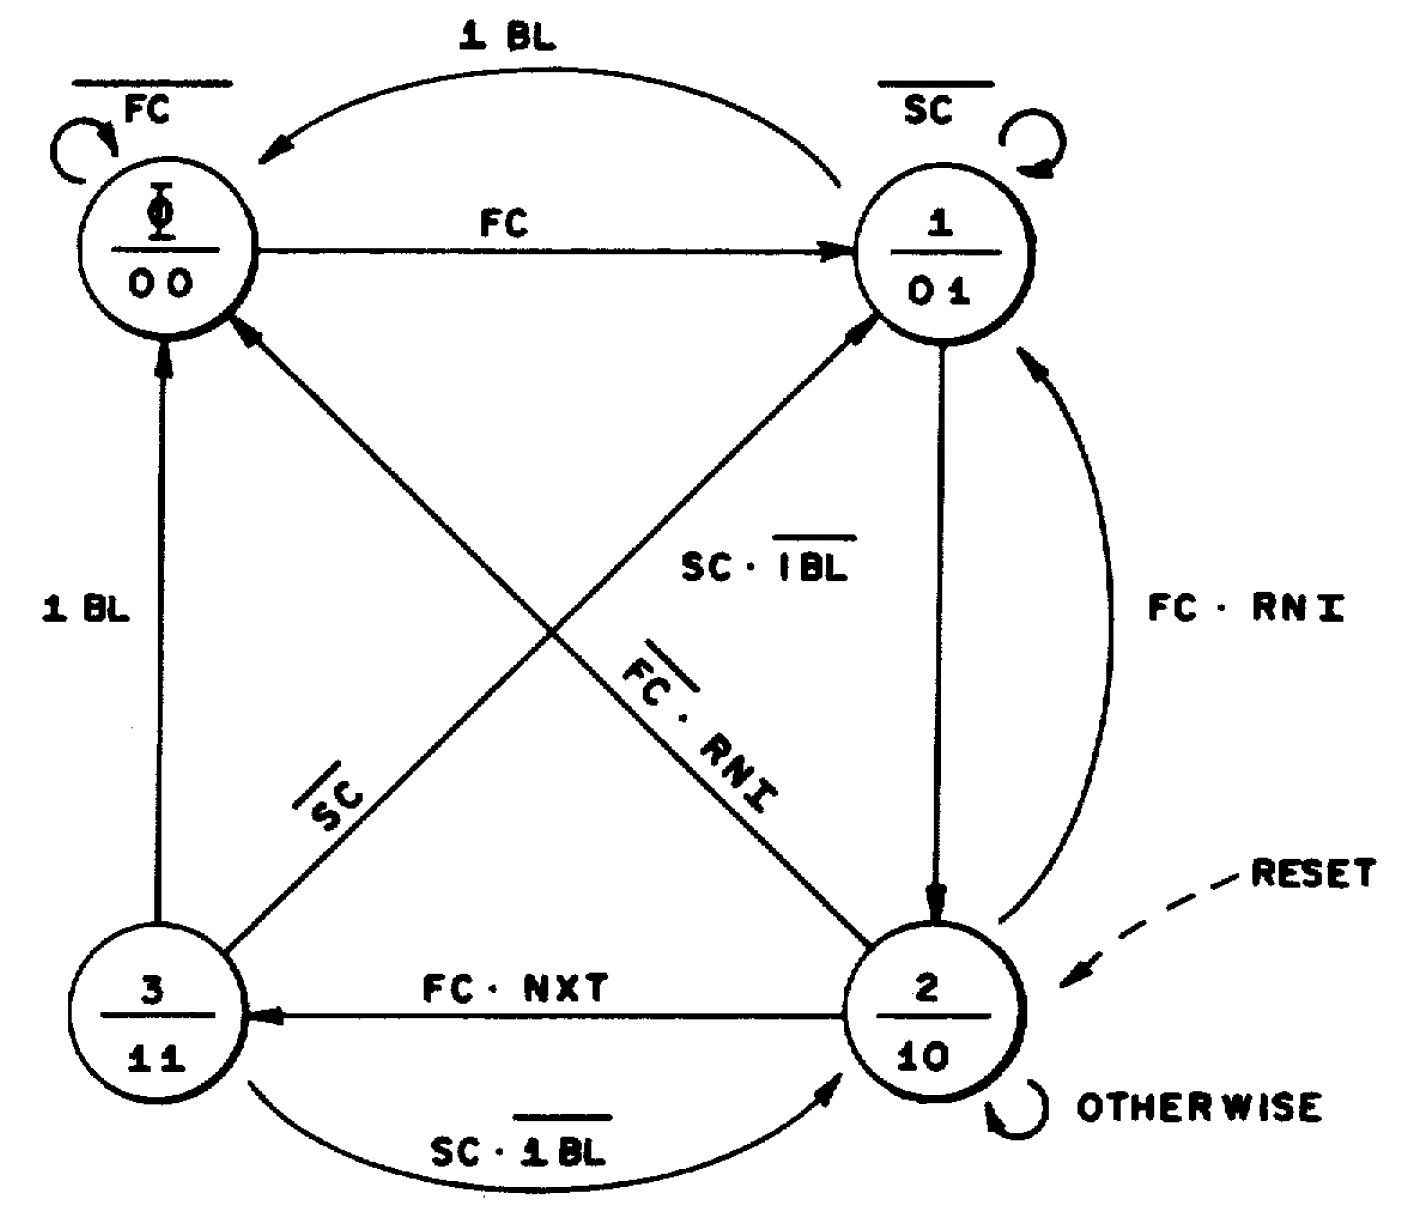
\includegraphics[width=0.8\textwidth]{files/8086.jpg}	
    \end{center}

\end{frame}


\section{\sc Chapter 1: Finite automata}


\section{1.1 Deterministic Finite Automaton}

	
\begin{frame}{Two simple examples}
    
    A finite automaton modeling an on/off switch.
	
    \begin{center}
        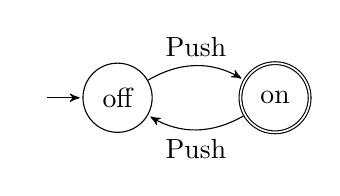
\begin{tikzpicture}[>=stealth',shorten >=1pt,auto,node distance=2cm]
    		\node[initial,state] (off)      {off};
    		\node[state,accepting]         (on) [right of=off]  {on};
    		\path[->] (off)  edge [bend left] node {Push} (on)
            (on) edge [bend left]  node {Push} (off);
        \end{tikzpicture}
    \end{center}

    A finite automaton modeling recognition of the word ``\alert{then}''.

	\begin{center}
        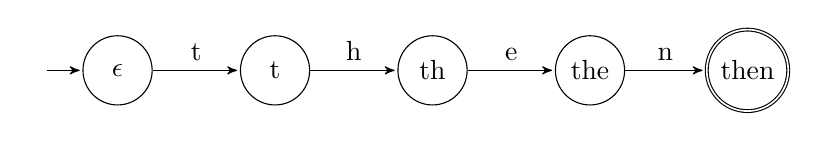
\begin{tikzpicture}[>=stealth',shorten >=1pt,auto,node distance=2cm]
        		\node[initial,state] (e)      {$\epsilon$};
        		\node[state] (t)  [right of=e]    {t};
        		\node[state] (th)  [right of=t]     {th};
        		\node[state] (the) [right of=th]     {the};
        		\node[state,accepting] [right of=the](then)      {then};
        		\path[->] (e)  edge  node {t} (t) 
                    (t)  edge  node {h} (th)
        			(th)  edge  node {e} (the)
        			(the)  edge  node {n} (then);
        \end{tikzpicture}
    \end{center}

\end{frame}


\begin{frame}{The definition}

    \begin{definition}[Deterministic Finite Automaton]

        A \alert{deterministic finite automaton (DFA)} is $A=(Q,\Sigma,\delta,q_0,F)$ consisting of:
        \begin{itemize}
            \item a finite nonempty set of \alert{states} $Q$
            \item a finite nonempty set of \alert{input symbols} $\Sigma$ (the \alert{input alphabet})
            \item a \alert{transition function} $\delta\colon Q \times \Sigma \rightarrow Q$ %(represented by arcs labelled by $\Sigma$)
            \item an \alert{initial (start) state} $q_0\in Q$
            \item a set of \alert{accepting  (final) states} $F\subseteq Q$
        \end{itemize}
    \end{definition}

\end{frame}


\begin{frame}{Remarks}

    \begin{itemize}
        \item Sometimes we allow $\delta$ to be a partial function. If needed, we can make $\delta$ total by adding a new "Fail" state and making it the target state for all missing transitions.
                
        \item Sometimes we require at least one accepting state. If $F=\emptyset$, we can add to $F$ and $Q$ a new "Final" state with no transitions from other states and $\delta(\text{"Final"}, s)=\text{"Final"}$ for all $s\in \Sigma$.
    \end{itemize}

    \vspace{-1.5cm}
    \begin{center}
        \scalebox{0.85}{
            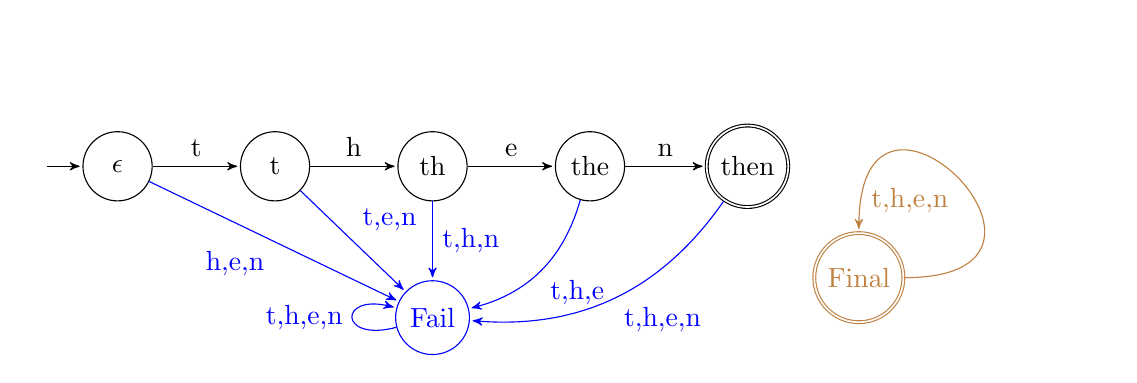
\begin{tikzpicture}[>=stealth',shorten >=1pt,auto,node distance=2cm]
                \node[initial,state] (e)      {$\epsilon$};
                \node[state] (t)  [right of=e]    {t};
                \node[state] (th)  [right of=t]     {th};
                \node[state] (the) [right of=th]     {the};
                \node[state,accepting] [right of=the](then)      {then};
                \node[state, color=blue] (fail) [below=1cm of th]     {Fail};
                \node[state, color=brown,accepting] (final) [below right of= then]     {Final};
                \path[->]
                    (e)  edge  node {t} (t)
                    (t)  edge  node {h} (th)
                    (th)  edge  node {e} (the)
                    (the)  edge  node {n} (then);
                \path[->,color=blue]
                    (e)  edge [swap]  node {h,e,n} (fail)
                    (t)  edge  node  {t,e,n} (fail)
                    (th)  edge node {t,h,n} (fail)
                    (the)  edge [bend left] node {t,h,e} (fail)
                    (then)  edge [bend left] node {t,h,e,n} (fail)
                    (fail)  edge [loop left] node {t,h,e,n} (fail);
                \path[->,color=brown] (final)  edge [in=90,out=0,loop] node {t,h,e,n} (final);
            \end{tikzpicture}
        }
    \end{center}
    
\end{frame}


\begin{frame}{Representing a DFA}

    \begin{example}
    A deterministic finite automaton $A$ that \alert{accepts} the language
    $L=\left\{  u01v\mid u,v\in\{0,1\}^* \right\}$.
    \end{example}

    \begin{itemize}
        \item the automaton: $A=(\{q_0,q_1,q_2\},\{0,1\},\delta,q_0,\{q_1\})$
        \item a \alert{state diagram}:        
        \begin{center}
            \scalebox{0.9}{
                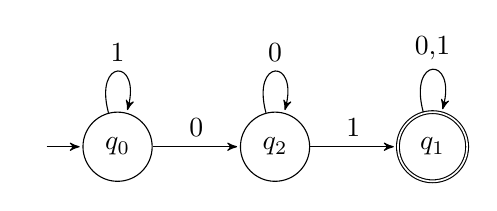
\begin{tikzpicture}[>=stealth',shorten >=1pt,auto,node distance=2cm]
                    \node[initial,state] (q0)      {$q_0$};
                    \node[state] (q2)  [right of=q0]     {$q_2$};
                    \node[state,accepting] (q1) [right of=q2]     {$q_1$};
                    \path[->]
                            (q0)  edge[loop above]  node {1} (q0)
                            (q0)  edge  node {0} (q2)
                            (q2)  edge[loop above]  node {0} (q2)
                            (q2)  edge  node {1} (q1)
                            (q1)  edge[loop above]  node {0,1} (q1);
                \end{tikzpicture}
            }
        \end{center}            
        \item a \alert{transition table}:        
        \begin{center}
            \begin{tabular}{r||c|c} 
                $\delta$ & 0 & 1\\ \hline \hline		
                $\rightarrow q_0$ & $q_2$ & $q_0$\\ \hline 
                $*q_1$ & $q_1$ & $q_1$\\ \hline 
                $q_2$ & $q_2$ & $q_1$
            \end{tabular}
        \end{center}
    \end{itemize}
    
\end{frame}


\section{1.2 Regular Languages}


\begin{frame}{Words and languages}

    \begin{itemize}
        \item an \alert{alphabet} $\Sigma$ is a finite nonempty set of symbols (letters)
        \item a \alert{word} $w$ over $\Sigma$ is a finite sequence of symbols from $\Sigma$
        \item that includes the \alert{empty word}, denoted by \alert{$\epsilon$} (or sometimes $\lambda$)
        \item \alert{$\Sigma^*$} denotes the set of all words over $\Sigma$, and $\alert{\Sigma^+}=\Sigma^*\setminus \{\epsilon\}$
        \item a \alert{language} $L\subseteq \Sigma^*$ is any set of words over the alphabet $\Sigma$
    \end{itemize}
          
    Note the difference: $L=\emptyset$ vs. $L'=\{\epsilon\}$.

    Operations on words from $\Sigma^*$:
    \begin{itemize}
        \item \alert{concatenation:} $u.v$ or $uv$
        \item \alert{powers:} $u^n$ ($u^0=\epsilon$, $u^1=u$, $u^{n+1}=u^n.u$)
        \item \alert{length:} $|u|$ ($|\epsilon|=0$, $|\text{banana}|=6$)
        \item \alert{number of occurences} of $s\in \Sigma$ in $u$: $|u|_s$ ($|banana|_a=3$)
    \end{itemize}

\end{frame}
   

\begin{frame}{Extended transition function}

    Start in a state $q\in Q$ and read a \cancel{letter $a\in \Sigma$} \alert{word $w\in \Sigma^*$}.

    \begin{definition}[Extended transition function]
        The \alert{extended transition function } $\delta^*\colon Q\times \Sigma^*\rightarrow Q$:

        \begin{itemize}
            \item $\delta^*(q,\epsilon)=q$ for all $q\in Q$ \hfill (base case)
            \item $\delta^*(q,ua)=\delta(\delta^*(q,u),a)$ for $q\in Q,u\in \Sigma^*,a\in \Sigma$ \hfill (induction)
        \end{itemize}

        (We will sometimes write $\delta$ in place of $\delta^*$.)
    \end{definition}

    \begin{example}
        $\delta^*(q_0,1100)=q_2$, $\delta^*(q_0,1100111111111001)=q_1$ 
    \end{example}
    \begin{center}
        \scalebox{0.9}{
            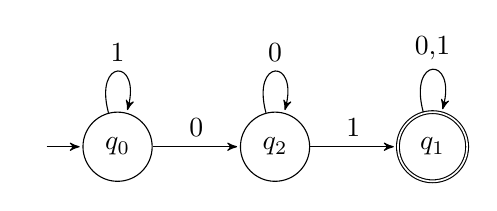
\begin{tikzpicture}[>=stealth',shorten >=1pt,auto,node distance=2cm]
        		\node[initial,state] (q0)      {$q_0$};
        		\node[state] (q2)  [right of=q0]     {$q_2$};
        		\node[state,accepting] (q1) [right of=q2]     {$q_1$};
        		\path[->]
        			(q0)  edge[loop above]  node {1} (q0)
        			(q0)  edge  node {0} (q2)
        			(q2)  edge[loop above]  node {0} (q2)
        			(q2)  edge  node {1} (q1)
        			(q1)  edge[loop above]  node {0,1} (q1);
        	\end{tikzpicture}
        }
    \end{center}

\end{frame}


\begin{frame}{Language recognized by an automaton}
    
    \begin{definition}[Language of a DFA]
        The language of the DFA $A$ is: 
        $$
        \alert{L(A)}=\{w\mid\delta^*(q_0,w)\in F\}
        $$
        \begin{itemize}
        \item a word $w$ is \alert{accepted [recognized]} by $A$, if $w\in L(A)$
        \item a language $L$ can be \alert{recognized} by a DFA, if there exists a DFA $A$ such that $L=L(A)$
        \item languages recognized by DFAs are called \alert{regular languages}
        \end{itemize}
    \end{definition}   

\end{frame}


\begin{frame}{Examples of regular languages 1/3}

    \begin{example}
        $L=\{w\in \{0,1\}^* \mid w=xux \text{ for some }x\in \{0,1\},u\in \{0,1\}^*\}$
    \end{example}

    \begin{center}
        \scalebox{0.9}{
            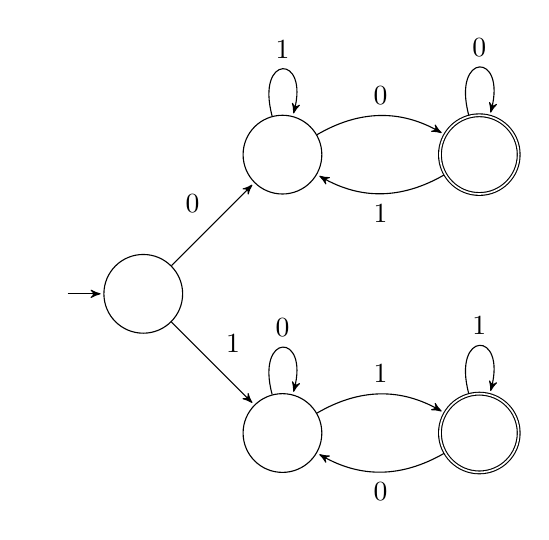
\begin{tikzpicture}[>=stealth',shorten >=1pt,auto, inner sep=0pt,minimum size=0.5cm, node distance=2.5cm]
                \tikzset{every state/.style={minimum size=1cm}}
                \node[initial,state] (s)      {};
                \node[state] (h1)  [above right of=s]    {};
                \node[state,accepting] (h2)  [right of=h1]     {};
                \node[state] (d1)  [below right of=s]    {};
                \node[state,accepting] (d2)  [right of=d1]     {};
                \path[->]
                    (s)  edge  node {0} (h1)
                    (s)  edge  node {1} (d1)
                    (h1)  edge [loop above] node {1} (h1)
                    (h1)  edge [bend left] node {0} (h2)
                    (h2)  edge [bend left] node {1} (h1)
                    (h2)  edge [loop above] node {0} (h2)
                    (d1)  edge [loop above] node {0} (d1)
                    (d1)  edge [bend left] node {1} (d2)
                    (d2)  edge [bend left] node {0} (d1)
                    (d2)  edge [loop above] node {1} (d2)
                ;
            \end{tikzpicture}
        }
    \end{center}	

\end{frame}


\begin{frame}{Examples of regular languages 2/3}

    \begin{example}
        $L=\{w\mid w=ubaba,u\in \{a,b\}^*\}$
    \end{example}
	
    \begin{center}
        \scalebox{1}{
            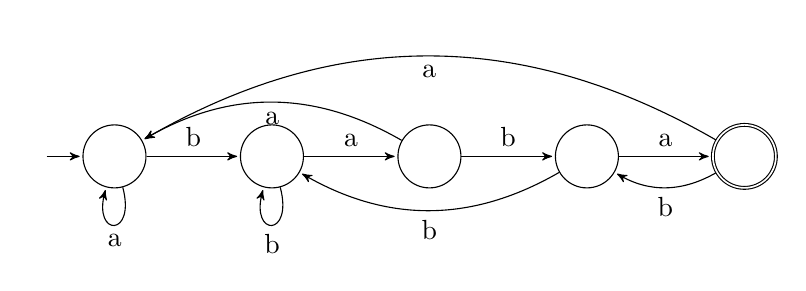
\begin{tikzpicture}[>=stealth',shorten >=1pt,auto,node distance=2cm]
                \tikzset{every state/.style={minimum size=0.8cm}}
                \node[initial,state] (a)      {};
                \node[state] (b)  [right of=a]     {};
                \node[state] (c) [right of=b]     {};
                \node[state] (d) [right of=c]     {};
                \node[state,accepting] [right of=d](e)      {};
                \path[->]
                        (a)  edge [loop below]  node {a} (a)
                        (a)  edge  node {b} (b)
                        (b)  edge [loop below] node {b} (b)
                        (b)  edge  node {a} (c)
                        (c)  edge [bend right] node {a} (a)
                        (c)  edge  node {b} (d)
                        (d)  edge [bend left] node {b} (b)
                        (d)  edge  node {a} (e)
                        (e)  edge [bend left] node {b} (d)
                        (e)  edge [bend right] node {a} (a)
                ;
            \end{tikzpicture}
        }
    \end{center}

\end{frame}


\begin{frame}{Examples of regular languages 3/3}

    \begin{example}
        $L=\{w\in \{0,1\}^*\mid w$ is the binary encoding of a positive integer divisible by 5$\}$
    \end{example}
	
    \begin{center}
        \scalebox{0.9}{
            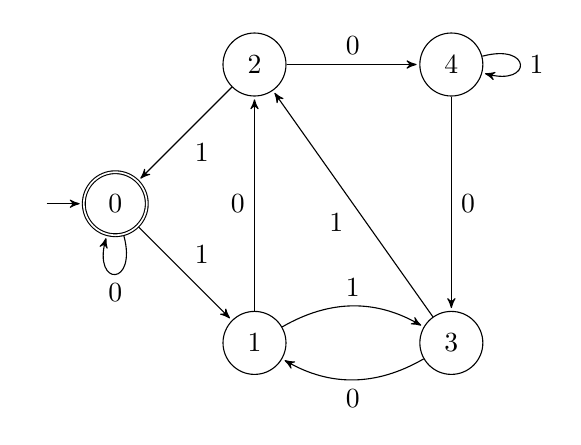
\begin{tikzpicture}[>=stealth',shorten >=1pt,auto,node distance=2.5cm]
                \tikzset{every state/.style={minimum size=0.8cm}}
                \node[initial,state,accepting] (a)      {0};
                \node[state] (b)  [below right of=a]     {1};
                \node[state] (c) [above right of=a]     {2};
                \node[state] (d) [right of=b]     {3};
                \node[state] [right of=c]   (e)   {4};
                \path[->]
                        (a)  edge [loop below]  node {0} (a)
                        (a)  edge  node {1} (b)
                        (b)  edge node {0} (c)
                        (b)  edge [bend left] node {1} (d)
                        (c)  edge node {1} (a)
                        (c)  edge  node {0} (e)
                        (d)  edge [bend left] node {0} (b)
                        (d)  edge  node {1} (c)
                        (e)  edge [loop right] node {1} (e)
                        (e)  edge  node {0} (d)
                ;
            \end{tikzpicture}    
        }
    \end{center}

    \begin{exercise}
        Improve to disallow zeros at the beginning of nonzero numbers.
    \end{exercise}

\end{frame}


\begin{frame}{Product automaton}

    \begin{example}
        $L=\{w\in \{0,1\}^*\mid |w|_0=2k \text{ and }|w|_1=2\ell\text{ for some }k,\ell\geq 0\}$.        
    \end{example}

    \begin{columns}
        
        \column{0.5\textwidth}

        \begin{center}
            \scalebox{0.9}{
                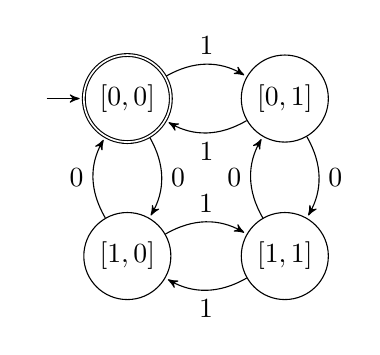
\begin{tikzpicture}[>=stealth',shorten >=1pt,auto,node distance=2cm]
                    \node[initial,state,accepting] (q0)      {$[0,0]$};
                    \node[state] (q2)  [below of=q0]     {$[1,0]$};
                    \node[state] (q3)  [right of=q2]     {$[1,1]$};
                    \node[state] (q1) [right of=q0]     {$[0,1]$};
                    \path[->]
                        (q0)  edge[bend left]  node {1} (q1)
                        (q1)  edge[bend left]  node {1} (q0)
                        (q1)  edge[bend left]  node {0} (q3)
                        (q3)  edge[bend left]  node {0} (q1)
                        (q3)  edge[bend left]  node {1} (q2)
                        (q2)  edge[bend left]  node {1} (q3)
                        (q2)  edge[bend left]  node {0} (q0)
                        (q0)  edge[bend left]  node {0} (q2)
                    ;
                \end{tikzpicture}
            }
        \end{center}

        \column{0.5\textwidth}

        \begin{center}
            \begin{tabular}{r||c|c}
        $\delta$ & 0 & 1\\ \hline \hline		
        $*\rightarrow [0,0]$ & $[1,0]$ & $[0,1]$\\ \hline 
        $[0,1]$ & $[1,1]$ & $[0,0]$\\ \hline 
        $[1,0]$ & $[0,0]$ & $[1,1]$\\ \hline 
        $[1,1]$ & $[0,1]$ & $[1,0]$
            \end{tabular}        
        \end{center}

    \end{columns}
    
    \begin{exercise}
        Formalize the construction of the product automaton.
    \end{exercise}
        
    \begin{corollary}
        If $L$ and $L'$ are regular, then $L\cap L'$ is also regular.
    \end{corollary}

\end{frame}


\section{1.3 Pumping Lemma}


\begin{frame}{A language that is not regular}

    \begin{example}
        $L=\{0^n1^n \mid  n\geq 0\}$ is not regular.
    \end{example}

    \begin{itemize}
        \item \alert{Intuition:} the automaton cannot `remember' arbitrarily large $n$ using only finitely many states    
    
        \item \alert{Formalization:} Pumping lemma
    \end{itemize}
    
\end{frame}


\begin{frame}{Pumping lemma}

    \begin{theorem}[Pumping Lemma For Regular Languages]
		Let $L$ be a regular language. Then there exists a constant $n\in \mathbb{N}$ (which depends on L) such that for every string $w\in L$ such that $|w|\geq n$, we can break $w$ into three strings, $w=xyz$, such that:
		
		\begin{itemize}
			\item $y\neq \epsilon$.
			\item $|xy|\leq n$.
			\item For all $k\geq 0$, the string $xy^kz$ is also in $L$.
		\end{itemize}
	\end{theorem}

    \textbf{Proof idea:} The constant $n$ is the number of states. Reading a word corresponds to a walk on the state diagram. Using the Pigeonhole principle, for long enough words we visit some state twice. The part of the walk between the first and second visit can be repeated (or skipped for $k=0$).

\end{frame}


\begin{frame}{Illustration: a regular language}

    \begin{center}
        \scalebox{1}{
            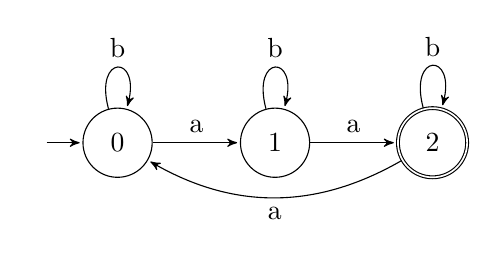
\begin{tikzpicture}[>=stealth',shorten >=1pt,auto,node distance=2cm]
                \node[initial,state] (a)      {0};
                \node[state] (b)  [right of=a]    {1};
                \node[state,accepting] [right of=b](c)      {2};
                \path[->]
                    (a)  edge  node {a} (b)
                    (b)  edge  node {a} (c)
                    (c)  edge [bend left]  node {a} (a)
                    (a)  edge [loop above] node {b} (a)
                    (b)  edge [loop above] node {b} (b)
                    (c)  edge [loop above] node {b} (c)
                ;
            \end{tikzpicture}
        }
    \end{center}

    \begin{itemize}
		\item \alert{$abbbba=a(b)bbba$}; for all $k\geq 0$ we have $a(b)^kbbba\in L(A)$
		\item \alert{$aaaaba=(aaa)aba$}; for all $k\geq 0$ we have $(aaa)^iaba\in L(A)$
		\item \alert{$aa$} cannot be pumped but it is too short: $|aa|<n=3$
	\end{itemize}

\end{frame}


\begin{frame}{Proof of the Pumping lemma}

    Suppose $L$ is regular, then $L=L(A)$ for some DFA $A$ with $n$ states.
        
    Take any word $w\in L$, $w=a_1a_2\ldots a_m$ of length $m\geq n$, $a_i\in \Sigma$. 
    
    Define $\forall i$ $p_i=\delta^*(q_0,a_1a_2\ldots a_i)$. Note $p_0=q_0$.
    
    We have $n+1$ $p_i$'s and $n$ states, therefore there are $i,j$ such that $0\leq i< j\leq n: p_i=p_j$.
    
    Define: $x=a_1a_2\ldots a_i$, $y=a_{i+1}a_{i+2}\ldots a_j$, $z=a_{j+1}a_{j+2}\ldots a_m$. Note $w=xyz$.
       
    \begin{center}
        \scalebox{0.8}{
            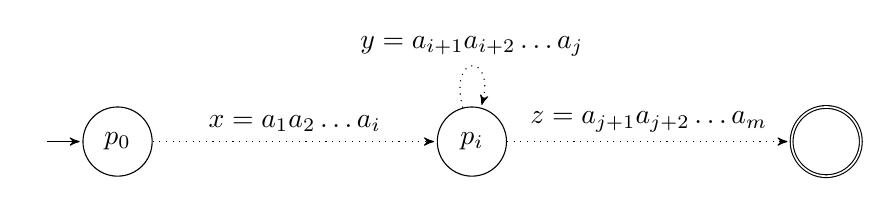
\begin{tikzpicture}[>=stealth',shorten >=1pt,auto,node distance=4.5cm]
                \node[initial,state] (q0)      {$p_0$};
                \node[state] (q1)  [right of=q0]     {$p_i$};
                \node[state,accepting] (q2) [right of=q1]     {};
                \path[dotted,->]
                    (q0)  edge  node {$x=a_1a_2\ldots a_i$} (q1)
                    (q1)  edge  node {$z=a_{j+1}a_{j+2}\ldots a_m$} (q2)
                    (q1)  edge[loop above]  node {$y=a_{i+1}a_{i+2}\ldots a_j$} (q1)
                ;
            \end{tikzpicture}
        }
    \end{center}
            

    The loop above $p_i$ can be repeated any number of times and the input is also accepted.\hfill\qedsymbol

\end{frame}


\begin{frame}{Application: proving nonregularity [an adversarial game]}

    \begin{example}
		The language $L_{eq}=\{w; |w|_0=|w|_1\}$ of all strings with an equal number of 0's and 1's is not a regular language.
	\end{example}
	\begin{proof}
        Suppose for contradiction that $L_{eq}$ is regular. Take $n$ from the pumping lemma.
        \begin{itemize}
            \item Pick $w=0^n1^n\in L_{eq}$.
            \item Break $w=xyz$ as in the pumping lemma, $y\neq \epsilon$, $|xy|\leq n$.
            \item Since $|xy|\leq n$ and it's at the beginning of $w$, it has only 0's. 
            \item The pumping lemma says: $xz\in L_{eq}$ (for $k=0$). However, it has less 0's and the same \# of 1's as $w$ so it's not in $L_{eq}$.
        \end{itemize} 
        \vspace{-24pt}  
	\end{proof}

\end{frame}


\begin{frame}{More applications}

    \begin{example}
		The language $L=\{0^i1^i; i\geq 0\}$ is not regular. (Same proof as the previous example.)
	\end{example}
	
	\begin{example}
		The language $L_{pr}$ of all prime-length strings of 1's is not regular.
	\end{example}
	\begin{proof}
	Suppose it were. Take the constant $n$ from the pumping lemma.
	\begin{itemize}
		\item Consider some prime $p\geq n+2$, let $w=1^p$.
		\item Break $w=xyz$ by the PL, let $|y|=m$. Then $|xz|=p-m$.
		\item By the PL, $xy^{p-m}z\in L_{pr}$. But $|xy^{p-m}z|=|xz|+(p-m)|y|=p-m+(p-m)m=(m+1)(p-m)$ which is not a prime (none of two factors are $1$).
	\end{itemize}
    \vspace{-24pt}
	\end{proof}

\end{frame}


\begin{frame}{Not a characterization of regular languages!}

    The Pumping Lemma is not a \alert{characterization} of regular languages. (It is only an implication, not an equivalence.)
    
    \begin{example}[Nonregular language that can be `pumped']
        The language $L=\{u\in\{a,b,c\}^*\mid u=a^+b^ic^i \text{ or } u=b^ic^j\}$ is not regular but the first symbol can be always pumped.
    \end{example}

    ($a^+$ means at least one $a$, notation from regular expressions)

    Why? We can use the \alert{Myhill--Nerode theorem} (later) which is a characterization or alternatively a `Pumping Lemma with \alert{pumping near the end}'.
    
    \begin{exercise}
        State and prove a pumping lemma with pumping near the end. 
    \end{exercise}    
    
\end{frame}


\begin{frame}{Pumping lemma and finiteness}
	
	\begin{theorem}
	A regular language $L$ is infinite if and only if there exists $u\in L; n\leq |u|<2n$, where $n$ is the constant from the PL.
	\end{theorem}
	\begin{proof}
        \alert{\Large$\Leftarrow$} If $(\exists u\in L)\ n\leq |u|<2n$, then we can pump: split $u=xyz$, $xy^iz\in L$ for all $i\in \mathbb{N}$. That gives us infinitely many words in $L$.\\	
        \alert{\Large$\Rightarrow$} If $L$ is infinite, then it must contain a word $w$ with $n\leq |w|$. If $|w|<2n$, then we are done. Otherwise, using the PL: $w=xyz$ and $x{y^0}z=xz\in L$, and we get a shorter word. If $2n\leq |xz|$, we shorten  $xz$  further (PL again). Each time we cut $\leq n$ symbols; thus we hit the interval $[n,2n)$.
	\end{proof}
	
	\begin{corollary}To check if a regular language is infinite it is sufficient to check a finite number of strings:  $\{u\mid n\leq |u|<2n\}$.
	\end{corollary}

\end{frame}


\begin{frame}{Summary of Lecture 1}

    \begin{itemize}
        \item  \alert{Deterministic Finite Automaton (DFA)}: $A=(Q,\Sigma,\delta,q_0,F)$
        \item Extended transition function $\delta^*$
        \item The language \alert{recognized} by the DFA $A$ is the language 
        $$
        L(A)=\{w\in \Sigma^* \mid \delta^*(q_0,w)\in F\}
        $$    
        \item Languages recognized by some DFA are called \alert{regular}
        \item Finite automata encode only finite information, but can recognize infinite languages
        \item Product automaton, intersection of reg. languages is regular   
        \item \alert{Pumping lemma for regular languages} (prove nonregularity)
        \item PL not a characterization, some nonregular can be pumped
        \item A regular language is infinite iff it contains a word of length $n\leq |w|\leq 2n$ where $n$ is \#states of a recognizing automaton
    \end{itemize}

\end{frame}


\section{Appendix: A toy application}


\begin{frame}{Example of a (bad) electronic-money protocol}

    \begin{itemize}
        \item Three parties: the customer, the store, the bank.
        \item Only one 'money' file (for simplicity).    
        \item Customer may decide to transfer money to the store, which will the redeem the file from the bank and ship goods to the customer. The customer has the option to cancel the file.        
        \item Five events:
        \begin{itemize}
            \item Customer may \textbf{pay}.
            \item Customer may \textbf{cancel}.
            \item Store may \textbf{ship} the goods to the customer.
            \item Store may \textbf{redeem} the money.
            \item The bank may \textbf{transfer} the money by creating a new, suitably encrypted money file and sending it to the store.
        \end{itemize}
    \end{itemize}

    {\footnotesize\it [Hopcroft et al: Introduction to automata theory, languages, and computation]}
    
\end{frame}


\begin{frame}{(Incomplete) finite automata for the bank example}
     
    \begin{minipage}{\linewidth}
          \centering
    \begin{figure}[H]
        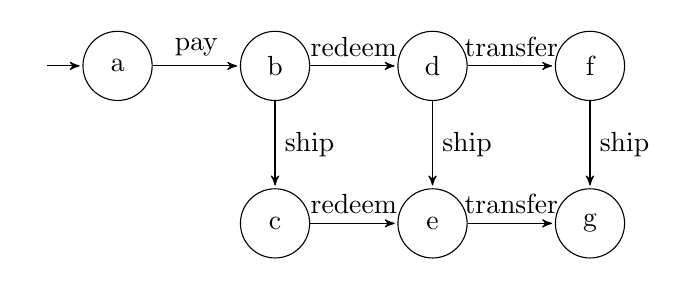
\begin{tikzpicture}[>=stealth',shorten >=1pt,auto,node distance=2cm]
                \node[initial,state] (a)      {a};
                \node[state] (b)  [right of=a]    {b};
                \node[state] (d)  [right of=b]     {d};
                \node[state] (f) [right of=d]     {f};
                \node[state] (c)  [below of=b]    {c};
                \node[state] (e)  [right of=c]     {e};
                \node[state] (g) [right of=e]     {g};
    %			\node[state,accepting] [right of=the](then)      {then};
            \path[->]
                    (a)  edge  node {pay} (b)
                    (b)  edge  node {redeem} (d)
                    (d)  edge  node {transfer} (f)
                    (d)  edge  node {ship} (e)
                    (b)  edge  node {ship} (c)
                    (f)  edge  node {ship} (g)
                    (c)  edge  node {redeem} (e)
                    (e)  edge  node {transfer} (g);
            \end{tikzpicture}
                 \caption{Store}
              \end{figure}
          \end{minipage}
    \begin{minipage}{\linewidth}
          \centering
          \begin{minipage}{0.35\linewidth}
              \begin{figure}[H]
        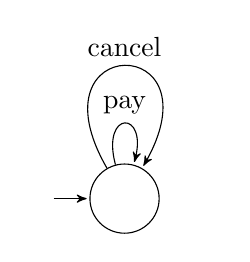
\begin{tikzpicture}[>=stealth',shorten >=1pt,auto,node distance=2cm]
                \node[initial,state] (a)      {};
            \path[->]
                    (a)  edge[loop above]  node {pay} (a);
    %				(a)  edge[loop above,min distance=10mm,in=0,out=60,looseness=10]  node {cancel} (a);
    \path[->,min distance=2cm] (a)edge[in=60,out=120,above] node {cancel}(a);
            \end{tikzpicture}
                  \caption{Customer}
              \end{figure}
          \end{minipage}
          \hspace{0.05\linewidth}
          \begin{minipage}{0.55\linewidth}
              \begin{figure}[H]
        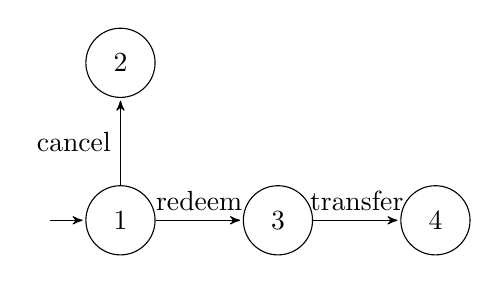
\begin{tikzpicture}[>=stealth',shorten >=1pt,auto,node distance=2cm]
                \node[initial,state] (1)      {1};
                \node[state] (2)  [above of=1]    {2};
                \node[state] (3)  [right of=1]     {3};
                \node[state] (4) [right of=3]     {4};
            \path[->]
                    (1)  edge  node {redeem} (3)
                    (3)  edge  node {transfer} (4)
                    (1)  edge  node {cancel} (2);
            \end{tikzpicture}
                  \caption{Bank}
              \end{figure}
          \end{minipage}
    \end{minipage}

\end{frame}
    

\begin{frame}{An edge for each Input}
    \begin{itemize}
        \item Formally, the automaton should perform an action for any input. The store automaton needs an additional arc from each state to itself, labeled {\it cancel}. 
        \item Customer mustn't kill the automaton by executing {\it pay} again, so loops labelled {\it pay} are necessary. Similarly other commands.
    \end{itemize}
    
    \begin{figure}[H]
        \begin{center}
            \scalebox{0.8}{
                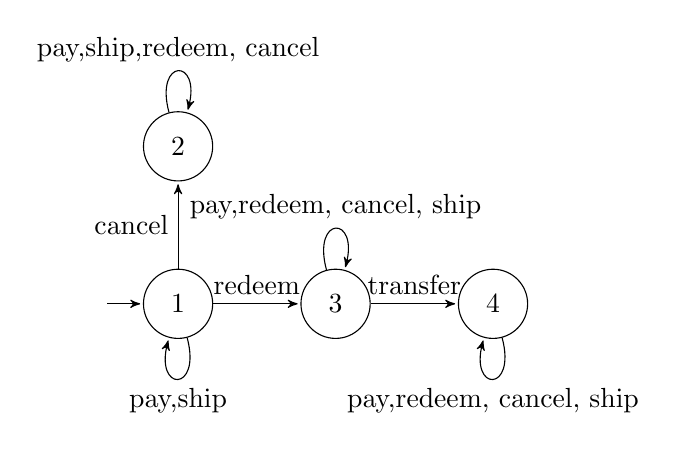
\begin{tikzpicture}[>=stealth',shorten >=1pt,auto,node distance=2cm]
                    \node[initial,state] (1)      {1};
                    \node[state] (2)  [above of=1]    {2};
                    \node[state] (3)  [right of=1]     {3};
                    \node[state] (4) [right of=3]     {4};
                    \path[->]
                        (2)  edge[loop above]  node {pay,ship,redeem, cancel} (2)
                        (1)  edge[loop below]  node {pay,ship} (1)
                        (3)  edge[loop above]  node {pay,redeem, cancel, ship} (3)
                        (4)  edge[loop below]  node {pay,redeem, cancel, ship} (4)
                        (1)  edge  node {redeem} (3)
                        (3)  edge  node {transfer} (4)
                        (1)  edge  node {cancel} (2)
                    ;
                \end{tikzpicture}
            }
        \end{center}        
        \caption{Extended Automaton for the Bank}
    \end{figure}

\end{frame}


\begin{frame}{Product automaton}
    
    The states of the product automaton of Bank and Store are pairs $B \times S$. To construct the arc of the product automaton, we need to run the bank and store automata 'in parallel'. If any automaton dies, the product dies too.

    \vspace{-12pt}

    \begin{columns}
        
        \column{0.6\textwidth}

        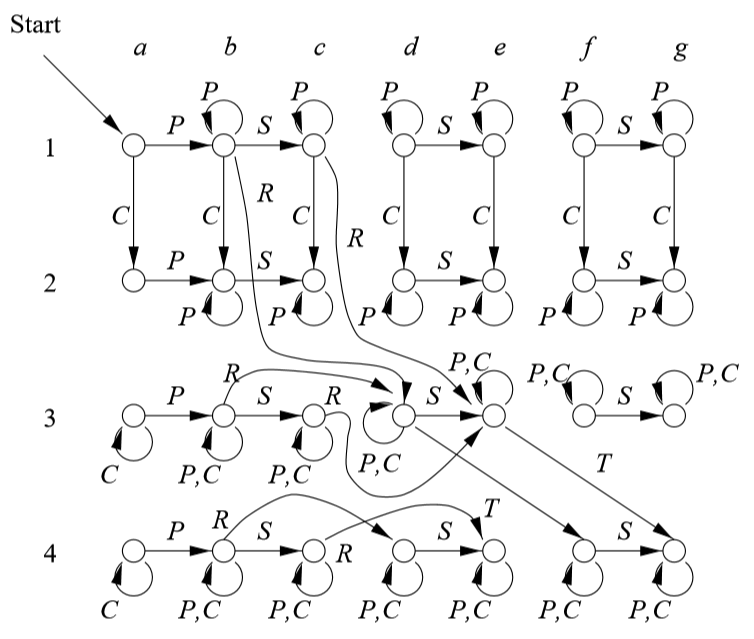
\includegraphics[width=\textwidth,keepaspectratio=TRUE]{files/product.PNG}

        \column{0.4\textwidth}

        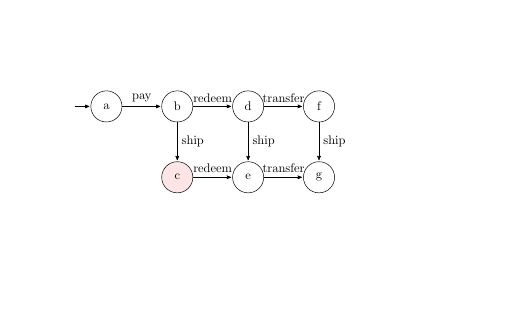
\begin{tikzpicture}[>=stealth',shorten >=1pt,auto,node distance=2cm]
            \useasboundingbox (-1,-2.50) rectangle (5,1);
            \scope[transform canvas={scale=.45}]
            \node[initial,state] (a)      {a};
            \node[state] (b)  [right of=a]    {b};
            \node[state] (d)  [right of=b]     {d};
            \node[state] (f) [right of=d]     {f};
            \node[state] (c)  [below of=b,fill=red!10]    {c};
            \node[state] (e)  [right of=c]     {e};
            \node[state] (g) [right of=e]     {g};
            % \node[state,accepting] [right of=the](then)      {then};
            \path[->]
                (a)  edge  node {pay} (b)
                (b)  edge  node {redeem} (d)
                (d)  edge  node {transfer} (f)
                (d)  edge  node {ship} (e)
                (b)  edge  node {ship} (c)
                (f)  edge  node {ship} (g)
                (c)  edge  node {redeem} (e)
                (e)  edge  node {transfer} (g)
            ;
            \endscope
        \end{tikzpicture}

        \begin{tikzpicture}[>=stealth',shorten >=1pt,auto,node distance=2cm]
            \useasboundingbox (-1,-2.50) rectangle (5,1);
            \scope[transform canvas={scale=.45}]
            \node[initial,state] (1)      {1};
            \node[state] (2)  [above of=1]    {2};
            \node[state] (3)  [right of=1]     {3};
            \node[state] (4) [right of=3]     {4};
            \path[->]
                (2)  edge[loop above]  node {pay,ship,redeem, cancel} (2)
                (1)  edge[loop below]  node {pay,ship} (1)
                (3)  edge[loop above]  node {pay,redeem, cancel, ship} (3)
                (4)  edge[loop below]  node {pay,redeem, cancel, ship} (4)
                (1)  edge  node {redeem} (3)
                (3)  edge  node {transfer} (4)
                (1)  edge  node {cancel} (2);
            \endscope
        \end{tikzpicture}

    \end{columns}

\end{frame}


\end{document}
